\documentclass[accepttest.tex]{subfiles}
\begin{document}
	\section{Indledning}
	\subsection{Formål}
	 Formålet med accepttesten er at opstille en række tests, specifikt udarbejdet til at verificere om de krav
	 der bliver fremvist i kravspecifikationen bliver opfyldt af produktet/prototypen. Dette gør det lettere hurtigt
	 at se om en given version af produktet/prototypen er tilfredsstillende.
	 \subsection{Referencer}
	  Accepttesten er opbygget ud fra de krav der er stillet af projektudbyderen (Preben Kidmose), samt
	  krav der løbende er opstået igennem udviklingen af produktet/prototypen. Disse krav er specificeret i dokumentet Kravspecifikation.
	  \subsection{Omfang og begrænsninger}
	  Accepttesten inderholder test af det samlede produkt og er den endelige
	  afprøvning af produktet.
	  \subsection{Godkendelseskriterier}
	  Accepttesten er afsluttet, når alle specificerede test cases er gennemført og godkendt.
	  Hvis der under accepttesten opstår fejl, der umuliggør fortsat udførsel af de efterfølgende test cases,
	  afbrydes accepttesten.
	  
	  Hvis der opstår fejl i enkelte test cases; men fortsat accepttest er mulig, underkendes den enkelte test og
	  accepttesten fortsætter med de næste test cases.
	  
	  Såfremt en test afbrydes eller en test case underkendes, skal der udfærdiges en problemrapport, der beskriver
	  årsagen til underkendelsen. Problemrapporten skal efterfølgende godkendes af både kunde og leverandør.

\subsection{Læsevejledning}
Dette dokument er bygget op af en række test-cases. Disse test-cases har til formål at verificere alle krav stillet i projektets kravspecifikation. De forskellige tests er bygget op med vejledning om hvordan de foretages. \textit{Forberedelse} beskriver hvordan systemet skal gøres klart før brug. \textit{Aktion} beskriver de handlinger der skal foretages for at udføre testen. \textit{Forventet resultat} beskriver det forventede resultat af testen. \textit{Accepteret} er til at notere om test-casen er godkendt eller afvist. 

Afsnittet performanceevaluering har til formål at teste systemets performance. Dette afsnit er ikke tilknyttet kravspecifikationen, da det ikke er bygget på krav fra projektudbyderen.
	  \pagebreak
\subsection{Test-rutiner}
Følgende rutiner beskrevet her vil blive refereret senere i accepttesten.
\subsubsection{Tal-test}
\label{taltest}
\begin{figure}
\centering
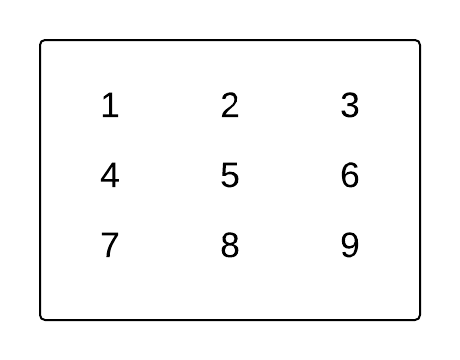
\includegraphics[width=0.5\linewidth]{Tal-test}
\caption{Layout af grafik på skærm for tal-testen.}
\label{fig:Tal-test}
\end{figure}
I denne test bliver testpersonen bedt om at fokusere på tallene i en bestemt rækkefølge. For eksempel $ 1,9,7,6,8,3\ldots $ Rækkefølgen bestemmes af brugeren. Herved kan den samme test gengives flere gange ved at genbruge samme talrække.

%\subsubsection{Krydsvalidering}
%$ DS 1 \rightarrow KAL 1 \rightarrow XY $ \hspace{2cm}
%$ DS 2 \rightarrow KAL 2 \rightarrow XY $ \\
%$ DS 1 \rightarrow KAL 2 \rightarrow XY $ \hspace{2cm}
%$ DS 2 \rightarrow KAL 1 \rightarrow XY $ \\
	  
\subsubsection{Dynamisk test}	  
\label{dyntest}
\begin{figure}
\centering
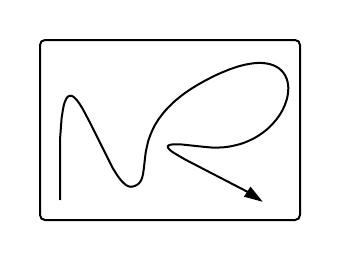
\includegraphics[width=0.4\linewidth]{DynamiskTest}
\caption{Eksempel på sti der skal følges ved dynamisk test.}
\label{fig:DynamiskTest}
\end{figure}
Ved dynamisk test bedes testpersonen om at følge en linje der bliver tegnet på skærmen. Denne test har til formål at vise hvor godt systemet kan foretage eye-tracking ved konstant bevægelse. 

\end{document}